\section{Audio}

 \begin{wrapfigure}{R}{0.4\textwidth}
	\vspace{-50pt}
	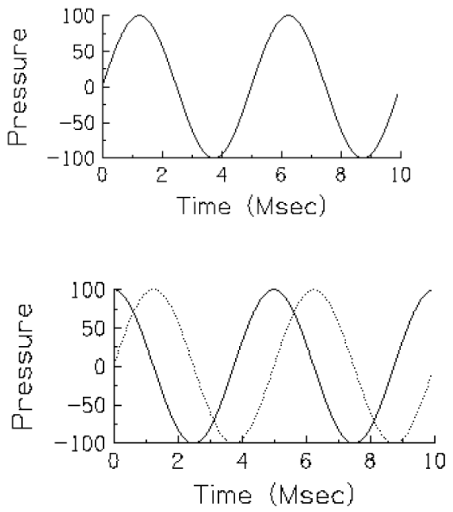
\includegraphics[width=0.4\textwidth]{Lezioni/Immagini/ondepressione}
	\vspace{-50pt}
\end{wrapfigure}

Un \textbf{segnale sonoro} è la variazione di pressione sul timpano, percepito nel tempo attraverso l'aria (mezzo di propagazione). 

Il suono è un'onda di pressione come la luce (fenomeno ondulatorio), ma macroscopico: le molecole dell'aria vengono compresse ed espanse, e la sorgente sonora vibra in modo longitudinale nella stessa direzione di propagazione del suono.
$$A(t) = A_{max} \cdot \sin(2\pi ft + \varphi_0)$$

I suoni elementari hanno andamento sinusoidale, periodico e con estensione indefinita. 

La maggior parte dei suoni natura sono caratterizzati da forme d'onda diverse, ma possono essere scomposte come una combinazione di suoni elementari.

Le componenti di un segnale sonoro sono individuate da:
\begin{itemize}
	\item \textit{Ampiezza} $A$, che si misura rispetto al valore medio della pressione dell'aria ed è espressa in dB;
	\item \textit{Periodo} $T$, la durata nel tempo di ogni ciclo dell'oscillazione, espresso in secondi;
	\item \textit{Frequenza} $F$, velocità con cui i valori di pressione fluttuano ciclicamente, espressa in numero di cicli al secondo (onde e Hz).
\end{itemize}

Il valore 0 indicato sull'asse della pressione corrisponde al valore medio della pressione nell'aria. La differenza di fase ha unicamente a che vedere con il fatto che due funzioni siano diversamente allineate rispetto al tempo.

\subsection{Analisi di Fourier}
L'analisi di Fourier permette la rappresentazione del segnale sonoro nel dominio delle frequenze a partire dal tempo, esplicitando $f$.

\begin{figure}[h]
	\centering
	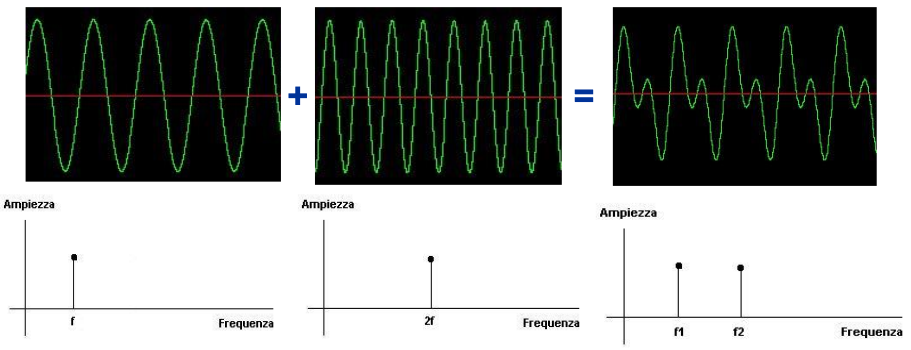
\includegraphics[scale=0.45]{Lezioni/Immagini/ondeverdi}
\end{figure}

La presenza di una linea nello spettro in frequenza indica la presenza di un segnale esattamente sinusoidale periodico, tuttavia i suoni caratterizzati da uno spettro discreto sono pochi. I suoni normalmente uditi hanno un inizio e una fine precisi, cioè sono contenuti in un intervallo temporale finito.

\begin{figure}[h]
	\centering
	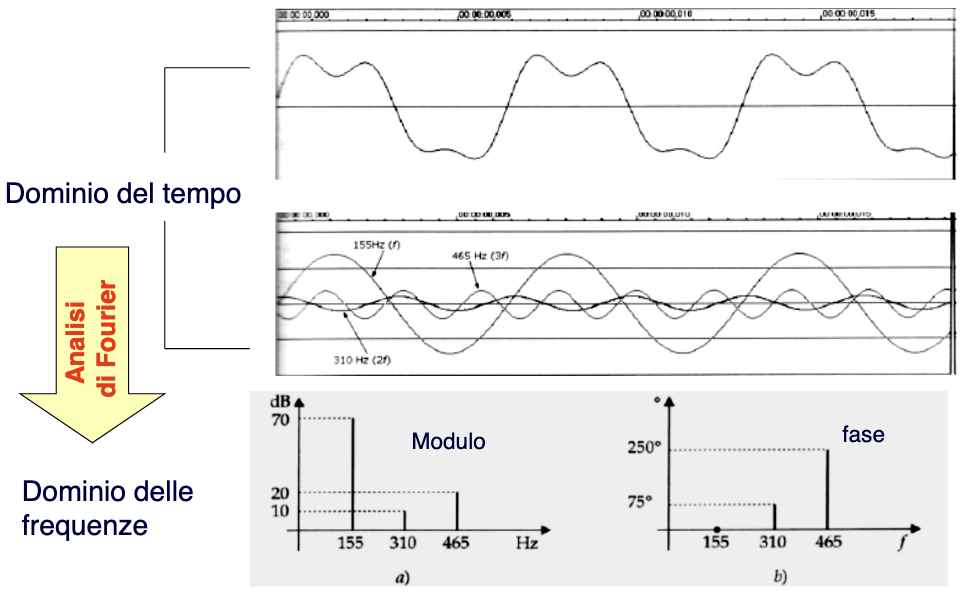
\includegraphics[scale=0.4]{Lezioni/Immagini/ondestorte}
\end{figure}

Ai parametri che descrivono un segnale ondulatorio possono essere associate le tre grandezze percettive che descrivono ogni suono:
\begin{itemize}
	\item \textbf{Altezza}, che rappresenta la tonalità dell'audio e ha come parametro la sequenza;
	\item \textbf{Intensità}, il volume, con parametro fisico l'ampiezza;
	\item \textbf{Timbro}, cioè la tipologia di strumento, con parametro fisico lo spettro.
\end{itemize}

A parità di frequenza fondamentale e intensità, \textit{due suoni possono differire per timbro} (la sovrapposizione delle onde sinusoidali può essere diversa).

\newpage
La frequenza fondamentale è proporzionale all'altezza del suono, cioè della sensazione di acutezza o gravità. L'aumento della frequenza non è linearmente in rapporto con l'ampiezza, ma si comporta seguendo una scala di tipo logaritmico. Affinché in un suono sia possibile individuare un'altezza, esso deve essere periodico. 

\subsection{Grandezze fisiche e grandezze percettive}

 \begin{wrapfigure}{L}{0.4\textwidth}
	\vspace{-15pt}
	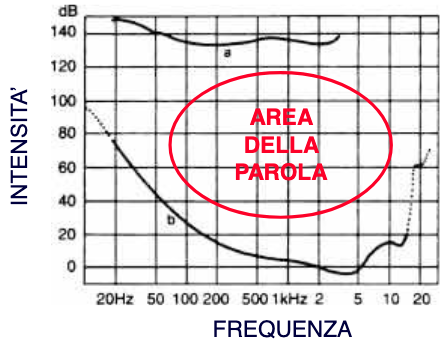
\includegraphics[width=0.4\textwidth]{Lezioni/Immagini/parola}
	\vspace{-40pt}
\end{wrapfigure}

Ampiezza e frequenza della forma d'onda hanno effetto sul suono percepito: variazioni di piccola ampiezza producono suoni di bassa intensità e viceversa, e al crescere della frequenza aumenta il tono (non linearmente).

Le energie in gioco nei fenomeni acustici sono irrilevanti rispetto a quelle nel fenomeno luminoso. 

Il range di suoni in grado di essere percepite dagli umani (tra i 20 e i 20.000 Hz) è minore dell'insieme delle frequenze possibili, oltre esso ci sono ultrasuoni e infrasuoni. 

Il volume aumenta man mano che l'ampiezza cresce, e l'incremento di tono è sempre più piccolo al crescere della frequenza.

Il \textbf{campo di udibilità} è determinato dai valori limite di intensità e frequenza. Il limite inferiore per l'intensità è costituito dalla curva di soglia di udibilità, mentre quello superiore dalla soglia del dolore. 

Le curve isofone rappresentano i suoni all'interno di una soglia di udibilità, che può essere superata fino al fastidio. Esse dipendono dall'intensità e dalla frequenza.

Vengono usate scale di rappresentazione che riflettono uguali differenze percettive. La \textit{scala di Mei} indica la relazione tra sensazione di altezza e frequenza: uguali differenze sulla scala corrispondono a uguali differenze percepite di tono, ma non di frequenza.

Le ampiezze sono rappresentate in scala logaritmica e hanno come unità di misura il dB. Incrementi di 1 dB corrispondono a JND (Just Noticeable Differences).

\subsection{Campionamento}
Le variazioni di pressione vengono tradotte in variazioni di tensione/corrente elettrica dal microfono, che effettua una \textit{trasduzione elettroacustica}. Il filtro antialiasing è applicato tramite amplificazione e filtraggio, per poi effettuare conversione A/D e registrazione su supporto.

La funzione a gradini generata dal convertitore viene filtrata con un filtro passa-basso prima del campionamento, per limitare le frequenze e l'aliasing. L'intervallo di frequenze che viene mantenuto dipende dall'applicazione.

Il segnale vocale può avere componenti fino a 10 KhZ, ma in genere se ne utilizzano solo 8, quindi questa è la frequenza di campionamento del segnale telefonico. Il segnale musicale ha range tra 20 Hz e 20 kHz.

Dopo la conversione DA, nell'output possono essere di nuovo presenti alte frequenze a causa del campionamento e della quantizzazione, quindi viene applicato un ulteriore filtro. La frequenza di campionamento standard è di 44,1 kHz, per registrare audio in formati differenti. Al di fuori di tale soglia si incorre in sovracampionamento o sottocampionamento (aliasing). 

La maggior parte dell'informazione del segnale vocale è contenuta in 4 kHz, ma esso andrebbe campionato a 40 kHz. Esiste anche per il campionamento il SNR (dB), con potenza del segnale proporzionale al quadrato della tensione.
$$SNR = 10\log_{10} \frac{V^2\text{segnale}}{V^2\text{rumore}} = 20\log_{10} \frac{V\text{segnale}}{V\text{rumore}}$$

\subsection{Dimensione e codifica}
Lo spazio in memoria (kB) occupato da un file audio si calcola con la seguente formula:
$$\frac{f_c \cdot D \cdot b \cdot N_c}{8 \cdot 1024}$$
$f_c$ è la frequenza di campionamento, $D$ è la durata in secondi, $b$ è il numero di bit del quantizzatore e $N_c$ è il numero di canali (mono o stereo).

I dati non compressi crescono al crescere della risoluzione del quantizzatore, dato che aumenta il numero di bit. Un segnale stereo raddoppia la banda per la trasmissione. 

La codifica può avvenire in due modi:
\begin{itemize}
	\item PCM (Pulse Code Modulation), modulazione del \textbf{codice} dell'impulso;
	\item PAM (Pulse Amplitude Modulation), modulazione dell'\textbf{ampiezza} dell'impulso.
\end{itemize}

La PCM converte in forma digitale i segnali analogici, trasformando le forma d'onda attraverso campionamento, quantizzazione e codifica. I valori numerici diventano e di 4 bit, e la rappresentazione può essere lineare o non.

Il trasmettitore digitale associa una forma d'onda a ogni cifra in uscita dal PCM, e all'uscita del canale le onde sono riconosciute dal ricevitore digitale e riconvertite nelle cifre originarie.

PAM è un modo per associare forme d'onda a simboli in uscita da una qualsiasi sorgente discreta. Essa prevede che si associ a ogni numero nella sequenza di bit la stessa pulsazione base, con un'ampiezza che dipende dal valore trasmesso.

I sistemi PAM inviano sul canale una sequenza di forme d'onda diverse tra loro, ma di diversa ampiezza. In ricezione, osservando l'ampiezza si può risalire al messaggio originale.

Nel processo di digitalizzazione, la qualità del suono è legata al tentativo di soddisfare due esigenze opposte:
\begin{enumerate}
	\item Fedeltà nella riproduzione;
	\item Dimensione del file.
\end{enumerate}

Le onde creano interferenze nello spazio, quindi è necessario creare l'effetto di più suoni generati in punti distinti e il numero di canali è un fattore importante. Le configurazioni più usate sono stereo e surround $5 + 1$, con 5 canali contenenti frequenze medie e alte, e un subwoofer per quelle basse. 

In fase di scrittura su disco, i campioni provenienti da diversi canali vengono trasmessi in successione. Questa tecnica si chiama \textit{interleaving}, o \textit{multiplexing} in caso di trasmissione. Al momento della riproduzione, occorre utilizzare buffer per la sincronizzazione.
